\documentclass[]{article}

\usepackage[utf8]{inputenc}
\usepackage[T1]{fontenc}
\usepackage[frenchb]{babel}
\usepackage{amsmath,amsfonts,amssymb,amsthm}
\usepackage{graphicx}

\begin{document}

    \begin{figure}[ht]
        \centering
        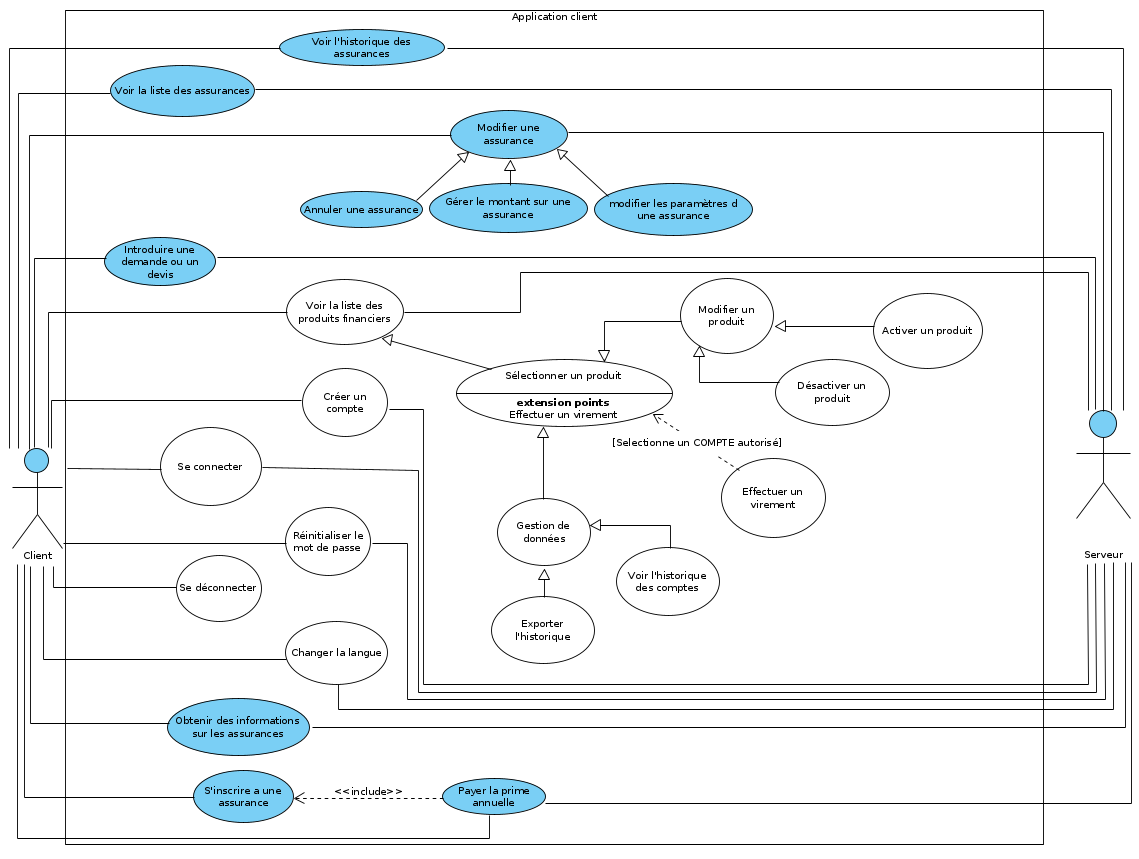
\includegraphics[scale=0.3]{img/UseCaseClient.png}
        \caption{Use case de l'application client}
        \label{fig1}
        \end{figure}

    \paragraph{}Le use case de l’extension assurance rajoute dix cas. Ceux si seront détaillés à part du rapport dans un fichier pdf qui reprend les descriptions semi-structurées. Il y a cependant quelques particularités comme le use case “Introduire une demande” qui a été modifié en “Introduire une demande ou un devis”, le use case “Modifier une assurance” qui comprend plusieurs spécifications et le use case “S’inscrire à une assurance” qui inclus “Payer la prime anuelle” car l’inscription se valide via le premier payement.


\end{document}